\documentclass[12pt]{article}
\usepackage[utf8]{inputenc}
\usepackage[margin=1in]{geometry}
\usepackage{amsmath,amssymb,multicol,enumitem}
\usepackage{pgfplots}\pgfplotsset{compat=1.17}
\setlength{\parindent}{0pt}
\begin{document}

\fbox{\parbox{0.97\linewidth}{\small\textbf{Final answers} (record here --- graded on the answer; show your work):\\[6pt]1.~\underline{\hspace{1.5cm}}\quad 2.~\underline{\hspace{1.5cm}}\quad 3.~\underline{\hspace{1.5cm}}\quad 4.~\underline{\hspace{1.5cm}}\quad 5.~\underline{\hspace{1.5cm}}}}
\vspace{0.35cm}

\begin{center}{\Large\textbf{Quadratic Functions: Vertex, Max \& Min}}\end{center}
\vspace{0.1cm}

\textbf{Example.}\ For $y=x^{2}-4$ the vertex is $(0,-4)$, a \textbf{minimum}. The graph \emph{decreases} for $x<0$ and \emph{increases} for $x>0$.\\[3pt]
\begin{center}
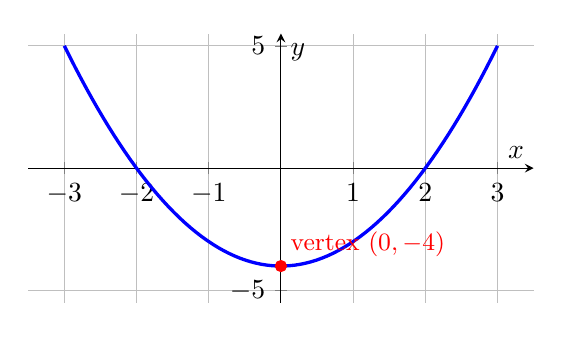
\begin{tikzpicture}
\begin{axis}[axis lines=middle,xlabel=$x$,ylabel=$y$,xmin=-3.5,xmax=3.5,ymin=-5.5,ymax=5.5,
  width=8cm,height=5cm,grid=both,samples=80]
\addplot[very thick,blue,domain=-3:3]{x^2-4};
\addplot[only marks,mark=*,red] coordinates {(0,-4)};
\node[above right,red,font=\small] at (axis cs:0,-4) {vertex $(0,-4)$};
\end{axis}
\end{tikzpicture}
\end{center}
\vspace{0.1cm}\hrule\vspace{0.35cm}

\textbf{Directions: for each function state max or min, give the vertex, and the increasing / decreasing intervals.}\\[6pt]
\begin{multicols}{2}
\begin{enumerate}[label=\textbf{\arabic*.},itemsep=2.4cm]
\item $y=x^{2}+2$
\item $y=-x^{2}+5$
\item $y=(x-3)^{2}$
\item $y=-(x+1)^{2}-2$
\end{enumerate}
\end{multicols}

\vspace{0.1cm}\hrule\vspace{0.3cm}
\textbf{Challenge}\ (same sheet):\\[4pt]
\begin{enumerate}[label=\textbf{\arabic*.},start=5,itemsep=2.2cm]
\item $y=(x-2)^{2}-9$ --- give the vertex, both intervals, \emph{and} the two $x$-intercepts.
\end{enumerate}

\newpage
\begin{center}{\Large\textbf{Answer Key --- fully worked}}\end{center}
\vspace{0.15cm}
\textbf{Procedure:}\ opens up ($+x^2$) $\Rightarrow$ minimum; opens down ($-x^2$) $\Rightarrow$ maximum. From $y=a(x-h)^2+k$ the vertex is $(h,k)$; the graph turns there.\\[8pt]
\begin{enumerate}[label=\textbf{\arabic*.},itemsep=8pt]
\item $y=x^{2}+2$: opens \textbf{up} $\Rightarrow$ \textbf{min}; vertex $(0,2)$; decreasing $x<0$, increasing $x>0$.
\item $y=-x^{2}+5$: opens \textbf{down} $\Rightarrow$ \textbf{max}; vertex $(0,5)$; increasing $x<0$, decreasing $x>0$.
\item $y=(x-3)^{2}$: vertex $(3,0)$, opens up $\Rightarrow$ \textbf{min}; decreasing $x<3$, increasing $x>3$.
\item $y=-(x+1)^{2}-2$: vertex $(-1,-2)$, opens down $\Rightarrow$ \textbf{max}; increasing $x<-1$, decreasing $x>-1$.
\item $y=(x-2)^{2}-9$: vertex $(2,-9)$ \textbf{min}; dec $x<2$, inc $x>2$; intercepts: $(x-2)^2=9\Rightarrow x-2=\pm3\Rightarrow x=-1,\ 5$.
\end{enumerate}
\end{document}
